\documentclass[finalReport.tex]{subfiles}
\begin{document}
\chapter{Implementation}

The main and more relevant aspects of the implementation of the server, the web application client and the android client are respectively presented in the Sections \ref{sec:impl:server}, \ref{sec:impl:web-app} and \ref{sec:impl:android}.

\section{Server}\label{sec:impl:server}
This Section describes the general implementation of the server. Figure \ref{Fig: server-methods} shows an overview on the interconnections between the implemented methods.  

\begin{figure}[h] 
\centering
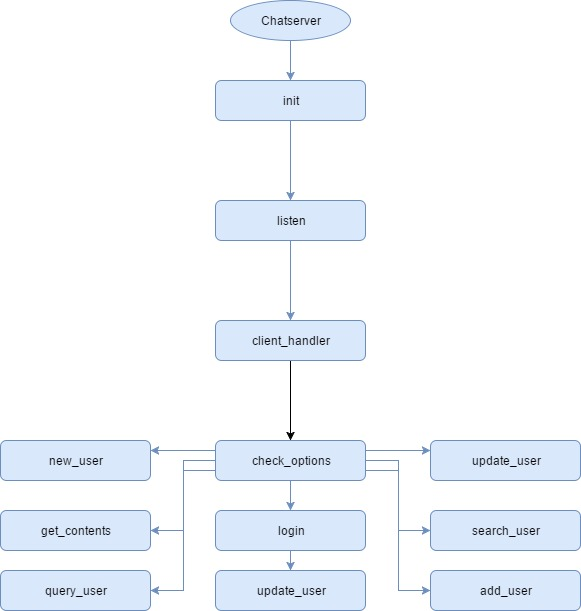
\includegraphics[scale=0.35]{Implementation/Plot/Server_methods.jpg}
\caption{Diagram of the connections between the Servers methods}\label{Fig: server-methods}
\end{figure}

The implementation of the functional requirements began with the implementation of a TCP server as this was the fundamental component on which other requirements and tests were based on. The server was implemented in python with IPv4 TCP sockets. The sockets were implemented with the use of python's socket library. Primarily through python's \lstinline'socket()' function, which allowed the project team to implement the various socket system calls. 

For example, as is seen in the source code:

\begin{lstlisting}
self.sock = socket.socket(socket.AF_INET, socket.SOCK_STREAM)   #Create TCP socket
self.sock.setsockopt(socket.SOL_SOCKET, socket.SO_REUSEADDR, 1)
self.sock.bind((self.host, self.port))
\end{lstlisting}

The first python socket system call – \lstinline'socket.socket()' - creates the socket which is used for bidirectional communication at the network layer or layer 3. With the socket created, a socket option was applied to aid in better management of the socket connection. This was achieved with the \lstinline'setsockopt()' system call to set the option at the socket level specified by \lstinline'socket.SOL_SOCKET' option. The  \lstinline'socket.SO_REUSEADDR' flag was needed to prevent an operating system error known as ``\textit{OSError: [Errno 98] Address already is use}'' from occurring, as a result of running the program over and over in quick succession, especially during testing. This is because the previous execution left the socket in a \lstinline'TIME_WAIT' state, and could not be immediately reused. The \lstinline'SO_REUSEADDR' flag signals to the kernel to reuse a local socket in \lstinline'TIME_WAIT' state, without waiting for its natural timeout to expire.

The second socket system call – \lstinline'bind()' - was used to tie the socket to the system's IPv4 address. For simplicity, the system's default address is used and it is assumed that there is not more than one network interfaces. In that case the socket will then listen on all interfaces. The socket was also bound to port 5001 to listen for incoming TCP connections. Port 5001 is above 1024, or the reserved ports, and it is a rarely used port by other applications.

As noted from the team's \textit{GitHub} history, this server was initially realized via a functional implementation. This allowed the team to firstly understand socket operations and socket programming before converting the server to an object oriented design and implementation.

The object oriented implementation of the server consists of a single class and eleven class methods that helped to achieve the functional requirements. One of the methods to note is the \lstinline'listen' method. This method listens and accepts incoming TCP connections via python's \lstinline'listen()' and \lstinline'accept()' socket methods. The 's listen method was designed and implemented to spawn a new thread when a new TCP connection was accepted by the \textit{chatserver}'s \lstinline'listen' method. Threading was implemented using python's \lstinline'thread' module. By implementing threading, the project team was able to have several tasks or threads running at the same time on the server, i.e. allowing the server to listen and accept multiple connections as well as sending and receiving data from multiple clients that connected.  The thread method from python's \lstinline'thread' module as noted in the \lstinline'listen()' method of the server and highlighted below:

\begin{lstlisting}
thread.start_new_thread(self.client_handler,(connected_client, client_address))
\end{lstlisting}

it starts a new thread by calling the \lstinline'client_handler()' method upon each new connection. The \lstinline'client_handler()' was implemented to communicate (outside the main thread of the server) with connected clients.  One of the caveats of socket communication that was discovered is that data sent via sockets needed to be in a specific encoding, usually as bytes, in order to be sent and received. To address this requirement, JSON encoding from pythons \lstinline'json' module was used in the \lstinline'client_handler()' method. The following lines of code from the \lstinline'client_handler()' method illustrates how the project team implemented json decoding and encoding.

\begin{lstlisting}
received_dict = json.loads(received_data.decode('utf-8'))
result = json.dumps(result).encode('utf-8')
\end{lstlisting}

The main purpose of the server is to facilitate queries from users/clients which would allow the users/clients to find other users and communicate with them. In order to achieve this, the server needed to allow users/clients to establish a connection and be able to exchange data. As described above the project team implemented these requirements with the \lstinline'listen()' and \lstinline'client_handler()' methods.

For the server and clients to effectively communicate, the project team devised a message exchange schema to allow clients to make specific requests to the server. The schema was implemented in the form ``\textit{key : list of values}''. More specifically, it was implemented as a python dictionary, with the key representing what function each list of values represent. In addition, the list of values was also implemented as a dictionary. For example, \lstinline-'query': \{'OPTION': 'QUERY_USER','USER':username\}- represents the query function. In this example the server will query the database for the user specified by the username variable. The server was implemented to always check the \lstinline-'OPTION'- field via its \lstinline'check_options()' method which it uses to determine what is required by the client and which of its methods to call. This schema proved particularly useful later in the project, when additional options were required. It was extremely easy to add options and methods as additional requirements were introduced.

As noted earlier, with respect to the server's main purpose, in order to keep track of users who are online and their connection details such as IP addresses, a datastore was needed. The \lstinline'sqlite' database was chosen, primarily because of its ease of use and implementation: it is very lightweight and does not require a separate server process. The \lstinline'sqlite' database was implemented via method calls to python's \lstinline'sqlite3' module. Eight of the eleven \textit{chatserver} methods were implemented to perform CRUD functionalities on the sqlite database named \textit{chatserver.db}. The required CRUD functionality depended on the \lstinline-'OPTION'- specified by the client.




\section{Web Application Client}\label{sec:impl:web-app}
This Section describes the general implementation of the Web Application client. Figure \ref{Fig: Wamethods} shows an overview on the interconnections between the implemented methods.  

\begin{figure}[h] 
\centering
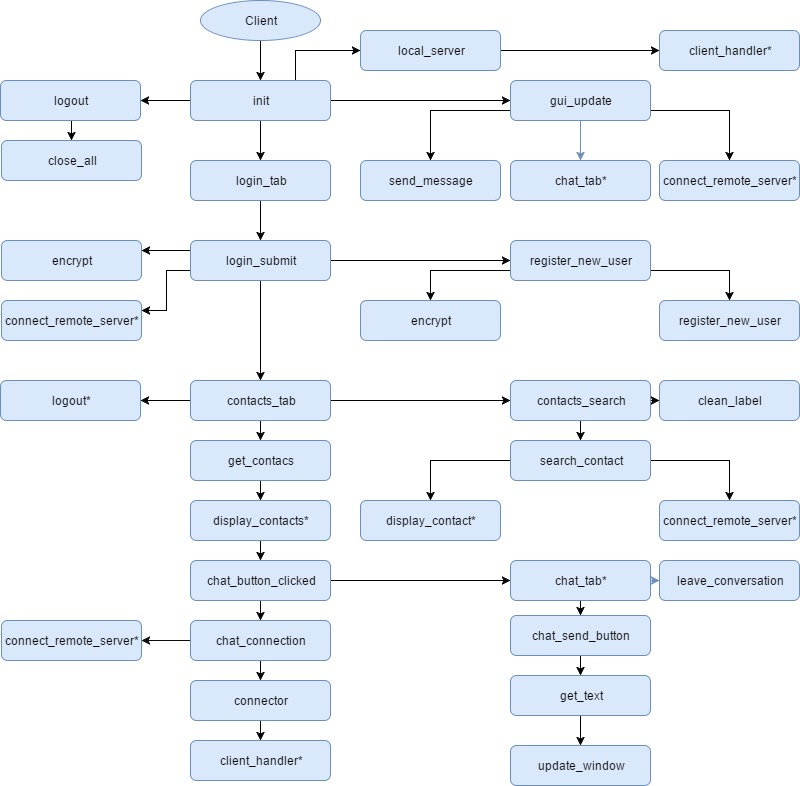
\includegraphics[scale=0.35]{Implementation/Plot/WAmethods.jpg}
\caption{Diagram of the connections between the Servers methods}\label{Fig: WAmethods}
\end{figure}



One of the functional requirement of the desktop client application is that users should be able to communicate with each other directly. This effectively meant that the application is a peer to peer application. The development of the application began with simultaneous implementation of the GUI, using python's \lstinline'tkinter' module, and the implementation of the socket/network functionality: the latter allows the client application to listen and accept connection from other clients, which is fundamentally the same requirement for the server. Since the desktop client was being implemented in python as well, the source code for the \textit{chatserver} formed the base code for the desktop client. Hence, the project team utilised the same \lstinline'listen()' method renamed \lstinline'local_server()', which is now started as a separate thread when the application starts, and \lstinline'client_handler()' method that were  described above.

The \lstinline'client_handler()' method was additionally modified to store all incoming messages into a FIFO queue. This means all received messages from users that the client is communicating with are entered into a queue, called \lstinline'received_messages'. The received messages queue was implemented as an object of python's \lstinline'queue' class from its \lstinline'queue' module. The \lstinline'queue' module implements multi-producer, multi-consumer queues. The following line in the modified \lstinline'client_handler()' method highlights how the project team achieved putting messages in the queue, with the \lstinline'put_nowait()' method of the queue object.

\begin{lstlisting}
self.received_messages.put_nowait(received_data)
\end{lstlisting}

The \lstinline'put_nowait()' method was used instead of the \lstinline'put()' to allow entering items into the queue without blocking. It was believed this was advantageous because of the small scale of the application.

As will be seen later on, the use of a queue is particularly useful for the spawned threads to exchange information themselves and the \lstinline'tkinter'-based GUI. The graphical user interface for the desktop application was implemented using python's \lstinline'tkinter' windowing toolkit. With the help of \lstinline'tkinter', the user interface was designed as a notebook with different tabs representing each action page of the chat application. The main tabs of the application are the \lstinline'login_tab' for logging in, the \lstinline'contacts_tab' for viewing the personal contact list and the \lstinline'chat_tabs' for having one to one conversations with contacts. The \lstinline'login_tab' shows two buttons associated to two different options - 'login' and 'register'. The client registration can be performed by selecting the register option that open up a registration window for submitting the username and password. The client encrypts the entered password and sends it along with the entered username to the remote server for registration. The password encryption functionality was implemented using the DES encryption standard from python's \lstinline'Crypto.Cipher' module which uses 8 bytes long block ciphers to generate encrypted password strings as illustrated below:

\begin{lstlisting}
des = DES.new('synomili', DES.MODE_ECB)
\end{lstlisting}


The \lstinline'tkinter''s notebook widget was utilized to achieve a tabbed window. 

\begin{lstlisting}
self.tab_controller = Notebook(self.demoPanel, name='notebook',width=420, height=550)
\end{lstlisting}

The above line of code illustrates how the project team implemented the tab window widget. One of the main reasons for implemented the notebook widget is that the user can communicate with several other users from the same window, just using different tabs. This was particularly significant from an implementation point of view, as the project team discovered that the behaviour of \lstinline'tkinter' windows became unreliable when updated from another thread. This is what led the team to implement queues for the exchange of messages. The design that followed was that all messages received were entered into the \lstinline'received_messages' queue as described above. Each message as part of the message exchange schema has a field for \lstinline-`USER'- which identifies who the message is from. This allows the application to know which tab to insert each message that is received, as each tab represents a different user with which the client is chatting.

This naturally leads us to a very significant method called \lstinline'gui_update()'. Show cased in the following code snippet, the application was implemented to extract from the \lstinline'received_messages' queue the message and the user from the message is. The program then proceeds to check if there is a tab already opened for that particular user, or proceeds to open one if none exists, and simply updates the existing tab for that user. In order to keep track of which tab belongs to which user, the project team utilises a dictionary (\lstinline'user_tabs_list') to maintain a map between remote users and the name of the tabs when they are created in the \lstinline'chat_tab()' method of the program. This is particularly important as without this mechanism the \lstinline'tkinter' window will not know which tab to update.


\begin{lstlisting}
try:            
    received_message = self.received_messages.get_nowait()
    user = received_message['USER']
    msg = received_message['MSG']            

    #Check if tab exists for user or not
    #Create new tab or update existing tab
    self.user_tabs_list
    if user not in self.user_tabs_list.keys():                    
        self.chat_tab(user)
		self.update_window(user,msg,False)
    else:
        self.update_window(user,msg,False)
except: 
    #Its ok if theres no data in the queue'
    #Will check again later'
     pass
\end{lstlisting}

The second part of the \lstinline'gui_update()' method was implemented to do the opposite of the first. Each message that is sent by the local user is placed in another queue used for outgoing messages called \lstinline'sent_messages'. The \lstinline'gui_update()' method retrieves each message from the queue and then extracts the name of the intended recipient. A lookup is then performed by the \lstinline'user_connection' dictionary which is used to maintain a mapping of each remote user and their sockets\footnote{This detail is added to the \lstinline'user_connection' dictionary when the user connects or a connection is initiated to the user}. The message to be sent and their socket information is passed to the \lstinline'send_message' method. This method was designed and implemented to connect to remote clients  and send the messages/data to them.

\begin{lstlisting}
try:            
	sent_message = self.sent_messages.get_nowait()
	#Check to see if the user is in the user_connection list            
	for key in self.user_connection.keys():           
	    if sent_message['USER'] ==  str(key):
	        #Get the connection string
	        connected_client = self.user_connection.get(key)                                
	        #encode the message as json and send
	        self.send_message(sent_message, connected_client)
except:
	#Its ok if theres no data in the queue
	#Will check again later
	pass
\end{lstlisting}


One of the most significant elements of the \lstinline'gui_update()' method implementation is the very last line:
\begin{lstlisting}
self.demoPanel.after(1000, self.gui_update)
\end{lstlisting}

The python \lstinline'after()' function was used to allow the \lstinline'gui_update()' method to call itself after a period of time. In this case, it is every 1000 milliseconds. This essentially means every second the \lstinline'gui_update()' method calls itself, checks both incoming and outgoing queues for messages and updates the tabs in the window if any new messages has arrived. It may not have been possible to implement a seemingly real time application in \lstinline'tkinter' without the after function.

-----------------------------------------------------------
(talk some more about tkinter???)


\section{Android Client}\label{sec:impl:android}







\end{document}